\synctex=1
%%%%%%%%%%%%%%%%                                ~~~~~~~~~~~~~~~~~~~~~~~~~~~~~~~~~~~~~~~~~~~~~~~~~~
% CONDITIONALS %
%%%%%%%%%%%%%%%%                                ~~~~~~~~~~~~~~~~~~~~~~~~~~~~~~~~~~~~~~~~~~~~~~~~~~

\newif\ifPeerReview\PeerReviewtrue              % Whether to create the PeerReview version or
                                                % Journal version
\newif\ifOnlineColor\OnlineColortrue            % Compile online color version?

\newif\ifFlatArchive\FlatArchivefalse           % Whether archive is flat (messy) or contain 
                                                % subfolders for graphics etc.
\newif\ifFloatAtEnd\FloatAtEndfalse             % Available in PeerReview mode:
                                                % Place floats at end of document?
\newif\ifTODO\TODOtrue                        % Use todo notes?

\newif\ifBuildBibliography\BuildBibliographyfalse  % Whether to include the references.bib file or use inline references.

\ifOnlineColor
   \newcommand\figPostfix{_online}              % Colored images online
\else
   \newcommand\figPostfix{_bw}                  % Black and white in journal
\fi

%%%%%%%%%%%%                                    ~~~~~~~~~~~~~~~~~~~~~~~~~~~~~~~~~~~~~~~~~~~~~~~~~~
% IEEEtran %
%%%%%%%%%%%%                                    ~~~~~~~~~~~~~~~~~~~~~~~~~~~~~~~~~~~~~~~~~~~~~~~~~~

\ifPeerReview
\documentclass[10pt,journal,draftclsnofoot,onecolumn]{IEEEtran}
% \newcommand\CLASSINPUTbaselinestretch{1.66}     % http://theoval.cmp.uea.ac.uk/~nlct/latex/thesis/node17.html
\else
\documentclass[journal]{IEEEtran}
\fi


%%%%%%%%%%%%%%%%%%%%%%%%%%                      ~~~~~~~~~~~~~~~~~~~~~~~~~~~~~~~~~~~~~~~~~~~~~~~~~~
% IEEE APPROVED PACKAGES %
%%%%%%%%%%%%%%%%%%%%%%%%%%                      ~~~~~~~~~~~~~~~~~~~~~~~~~~~~~~~~~~~~~~~~~~~~~~~~~~

\usepackage{cite}

\ifCLASSINFOpdf
   \usepackage[dvips]{graphicx}                 % Might not work. Use 'latex' instead of 
   \ifFlatArchive\else                          % 'pdflatex'
   \fi
\else
   \usepackage[dvips]{graphicx}
   \ifFlatArchive\else
   \fi
\fi

\RequirePackage[table,dvipsnames,svgnames]{xcolor}

\usepackage[cmex10]{amsmath}                    % cmex10 option to be IEEE explore compliant
\interdisplaylinepenalty=2500                   % Allows multiline equations to be broken

% \RequirePackage{amssymb}

\RequirePackage{array}

\ifCLASSOPTIONcompsoc
   \usepackage[caption=false,font=normalsize,labelfont=sf,textfont=sf]{subfig}
\else
   \usepackage[caption=false,font=footnotesize]{subfig}
\fi

% \usepackage{caption}
% \usepackage{subcaption}
\usepackage{color}
\usepackage{calc}
\usepackage{fp}


\ifFloatAtEnd
\ifCLASSOPTIONcaptionsoff                       % Places float at the end of the document when the
  \usepackage[nomarkers]{endfloat}              % captionsoff options is specified to IEEEtrans.cls
  \let\MYoriglatexcaption\caption               % (PeerReview mode)
  \renewcommand{\caption}[2][\relax]{\MYoriglatexcaption[#2]{#2}}
\fi
\fi

\usepackage{fixltx2e}                           % Fix some twocolumn float problems

% \usepackage{stfloats}                          % Allows: \begin{figure*}[!b]
                                                % (double column figures on top/bottom)

\usepackage{url}                                % Support for handling and breaking URLs

% NOTE: PDF hyperlink and bookmark features are not required in IEEE
%       papers and their use requires extra complexity and work.
% \newcommand\MYhyperrefoptions{bookmarks=true,bookmarksnumbered=true,
% pdfpagemode={UseOutlines},plainpages=false,pdfpagelabels=true,
% colorlinks=true,linkcolor={black},citecolor={black},urlcolor={black},
% pdftitle={Optimal Window Design for the Low Complexity Adaptive Beamformer in Active Sonar Imaging},
% pdfsubject={},
% pdfauthor={Jo Inge Buskenes},
% pdfkeywords={adaptive beamforming, beamforming, complexity, sonar, active}}%
\ifCLASSINFOpdf
%    \usepackage[\MYhyperrefoptions,pdftex]{hyperref}
   \usepackage[pdftex,
    final,                %Keep hyperlink stuff even when in draft mode
    breaklinks=true,      %Break links when necessary
    linktocpage=true,     %Enable link to page?
    linkcolor=black,  %Colour of links to labels within document
    citecolor=black,      %Colour of links to the biliography
    filecolor=red,        %Colour of links to local files
    pagecolor=black,        %Colour of links to other pages withing document
    urlcolor=Blue,        %Colour of the links to external URLs
    colorlinks=true,      %??
    plainpages=false,     %Store roman/arabic numbering differently to avoid
    bookmarksnumbered ]{hyperref}

\else
   \usepackage[\MYhyperrefoptions,breaklinks=true,dvips]{hyperref}
   \usepackage{breakurl}                        % Allows 'dvips' driver to break links
\fi

%%%%%%%%%%%%%%%%%%%%%%%                         ~~~~~~~~~~~~~~~~~~~~~~~~~~~~~~~~~~~~~~~~~~~~~~~~~~
% ADDITIONAL PACKAGES %       
%%%%%%%%%%%%%%%%%%%%%%%                         ~~~~~~~~~~~~~~~~~~~~~~~~~~~~~~~~~~~~~~~~~~~~~~~~~~


% \usepackage[maxfloats=40]{morefloats}
\newcounter{todoidx}
% \setcounter{todoidx}

\ifTODO
   \definecolor{todobackground}{rgb}{0.95,0.95,0.95}
   \setlength\marginparsep{1pt}
   \setlength\marginparwidth{35pt}
   \newlength\marginparwidthsmall
   \setlength\marginparwidthsmall{\marginparwidth}
   \addtolength\marginparwidthsmall{-7pt}
   \newcommand\todo[1]{%
      \addtocounter{todoidx}{1}%
      {\color{Red}\bf(\thetodoidx{})}%%\fbox{\bf\thetodoidx{}}}%
      \marginpar{%
         {\vspace*{-10pt}\color{Red}\fbox{\bf\thetodoidx{}}}\\%
         \fcolorbox{red}{todobackground}{\parbox{\marginparwidthsmall}{\raggedright\scriptsize #1}}}}

   \newcommand\todopar[1]{\fcolorbox{red}{white}{\parbox{0.97\linewidth}{#1}}}
\else
%    \usepackage[disable]{./todonotes} 
   \newcommand\todo[1]{}
\fi

\newenvironment{narrow}[2]{%
\begin{list}{}{%
\setlength{\topsep}{0pt}%
\setlength{\leftmargin}{#1}%
\setlength{\rightmargin}{#2}%
\setlength{\listparindent}{\parindent}%
\setlength{\itemindent}{\parindent}%
\setlength{\parsep}{\parskip}}%
\item[]}{\end{list}}

% \usepackage{float}

\ifOnlineColor
   \definecolor{tabBlue}{HTML}{AACCFF}
\else
   \definecolor{tabBlue}{HTML}{CCCCCC}
\fi

%%%%%%%%%%                                      ~~~~~~~~~~~~~~~~~~~~~~~~~~~~~~~~~~~~~~~~~~~~~~~~~~
% MACROS %       
%%%%%%%%%%                                      ~~~~~~~~~~~~~~~~~~~~~~~~~~~~~~~~~~~~~~~~~~~~~~~~~~

\newcommand\graphicsAI[2][]{%
  \immediate\write18{./bin/laFigure #2 #1}%
  \input{result}}%
  
% \DeclareMathOperator*{\argmin}{\text{arg}\;\text{min}}

\newcommand\Fig[1]{Fig.~\ref{#1}}
\newcommand\eq[1]{(\ref{#1})}

\newcommand\Grey[1]{{\color{Grey}#1}}
\newcommand\Red[1]{{\color{Red}#1}}
\newcommand\Blue[1]{{\color{Blue}#1}}
\newcommand\DarkBlue[1]{{\color{DarkBlue}#1}}
\newcommand\LightBlue[1]{{\color{LightBlue}#1}}
\newcommand\Brown[1]{{\color{Brown}#1}}
\newcommand\Green[1]{{\color{Green}#1}}
\newcommand\SeaGreen[1]{{\color{SeaGreen}#1}}
\newcommand\Yellow[1]{{\color{yellow}#1}}
\newcommand\Orange[1]{{\color{orange}#1}}

\newcommand\nn{\nonumber\\}

\newcommand\nmat[1]{\begin{matrix}#1\end{matrix}}
\newcommand\bmat[1]{\begin{bmatrix}#1\end{bmatrix}}
\newcommand\case[1]{\begin{cases}#1\end{cases}}
\newcommand\textbox[2]{\footnotesize\text{\parbox{#1}{\centering\emph{#2}}}}

\newcommand\rand{\text{rand}}
\newcommand\randn{\text{randn}}
\newcommand\rect{\text{rect}}
\newcommand\sinc{\text{sinc}}
\newcommand\tr{\text{tr}}
\newcommand\adj{\text{adj}}

% \newcommand\max{\text{max}}
\newcommand\argmin[1]{\text{arg}\;\underset{#1}{\text{min}}}

\newcommand\qqquad{\quad\qquad}
\newcommand\qqqquad{\qquad\qquad}

% \renewcommand\l[1]{\left#1}
% \renewcommand\r[1]{\right#1}

% {\text{\parbox{1.5cm}{\centering volume hyper- sphere}}}

%Keyword colouring:
\newcommand\kw[1]{#1}
\newcommand\parm[1]{#1}%\color{Black}#1\color{Black}}

\newcommand\of[1]{\scriptstyle(\parm{#1})\displaystyle}
\newcommand\df[1]{\scriptstyle[\parm{#1}]\displaystyle}
\newcommand\var[3]{#1_\text{#2}\of{#3}}

\newcommand\diag{\text{diag}}

% \raisebox{lift}[extend-above-baseline][extend-below-baseline]{text}
\newcommand\mt[1]{\text{\emph{#1}}} %mt = mathtext
\newcommand\mathnorm{\textstyle}
\newcommand\mathbig[1]{\displaystyle#1\mathnorm}
\newcommand\mathsmall[1]{\scriptstyle#1\mathnorm}
\newcommand\mathtiny[1]{\scriptscriptstyle#1\mathnorm}
\newcommand\sfrac[2]{\scriptstyle\raisebox{0.25pt}[0pt][0pt]{$\frac{#1}{#2}$}\mathnorm}
\newcommand\nfrac[2]{\textstyle\frac{#1}{#2}\displaystyle}

\newcommand\sumu[1]{\sum\limits^{#1}\;}
\newcommand\suml[1]{\sum\limits_{#1}\;}
\newcommand\sumb[2]{\sum\limits_{#1}^{#2}\;}

\newcommand\produ[1]{\prod\limits^{#1}\;}
\newcommand\prodl[1]{\prod\limits_{#1}\;}
\newcommand\prodb[2]{\prod\limits_{#1}^{#2}\;}

\newcommand\defeq{\overset{\underset{\mathrm{def}}{}}{=}}

%Math macros:
\newcommand\T{^{\scriptscriptstyle T}}
\renewcommand\H{^{\scriptscriptstyle H}}

\renewcommand\vec[1]{\boldsymbol{#1}}
\newcommand\mat[1]{\boldsymbol{#1}}

\newcommand\Om{O_\text{m}}
\newcommand\Oa{O_\text{a}}
\newcommand\Nl{N_\text{l}}
\newcommand\Nk{N_\text{k}}
\newcommand\1{\vec 1}
\newcommand\I{\mat I}
\renewcommand*\a{\vec a}
\newcommand*\f{\vec f}
\renewcommand*\i{\vec i}
\renewcommand*\k{\vec k}
\newcommand*\n{\vec n}
\newcommand*\p{\vec p}
\newcommand*\s{\vec s}
\newcommand*\w{\vec w}
\newcommand*\x{\vec x}
\newcommand*\y{\vec y}

\newcommand*\A{\mat A}
\newcommand*\B{\mat B}
\newcommand*\C{\mat C}
\newcommand*\E{\mat E}
\renewcommand*\P{\mat P}
\newcommand*\eP{\mat{\hat P}}
\newcommand*\R{\mat R}
\newcommand*\Ri{\R^{-1}}
\newcommand*\eR{\mat{\hat R}}
\newcommand*\eRi{\hat{\mat R}\;\!^{-1}}
\newcommand*\Navg{N_\text{avg}}
\newcommand*\W{\mat W}
\newcommand*\X{\mat X}
\newcommand*\Xd{\X_{\!\Delta}}
\newcommand*\Y{\mat Y}

\renewcommand\argmin{\text{argmin}}


\renewcommand*\P{\mat P}
\newcommand*\V{\mat V}
\newcommand*\M{\mat M}

\renewcommand*\L{\mat \Lambda}
\newcommand*\U{\mat U}
% \renewcommand*\t{\mathtiny{^T}}
% \newcommand*\h{\mathtiny{^H}}
\renewcommand*\t{^T}
\newcommand*\h{^H}

\newcommand\minus{\scalebox{0.75}[1.0]{$-$}}

% \usepackage{tikz}
% \usetikzlibrary{shapes,snakes}
\usepackage{amsmath,amssymb}
% \usepackage{datatool}
% \usepackage{glossaries}

% \newenvironment{outline}
% {\begin{itemize}}
% {\end{itemize}}
% 

\ifPeerReview
\graphicspath{./submission/submit1}
\fi

% \newcommand\multimedia[1]{\textbf{{\color{red}[#1]}}}
\newcommand\multimedia[2]{\href{#1}{#2}}

% \newcommand\mediaPath{gfx/media}
\newcommand\articlePath{http://folk.uio.no/joibu/articles/2015_JOE_LCA}

\newcommand\mediaI{\multimedia{\articlePath/media1.mp4}{Media Movie~1}}
\newcommand\mediaII{\multimedia{\articlePath/media2.mp4}{Media Movie~2}}


\begin{document}



\title{A Real-Time Sonar Simulator for Automatic Target Recognition}

\author{{Jo~Inge~Buskenes,~\IEEEmembership{Student Member,~IEEE,} %
        Herman~Midelfart, %
        \O{}ivind~Midtgaard} %
\thanks{J. I. Buskenes is with the Department of Informatics, University of Oslo, Norway.}%
\thanks{H. Midelfart and \O. Midtgaard are with The Norwegian Defence Research Establishment (FFI), Norway.}% <-this % stops a space
% \thanks{Manuscript received April 19, 2005; revised January 11, 2007.}
}

% The paper headers
\markboth{IEEE Journal of Oceanic Engineering}%
{A GPU Sonar Simulator for Automatic Target Recognition}

% Publishers ID mark:
%\IEEEpubid{0000--0000/00\$00.00~\copyright~2007 IEEE}

% use for special paper notices
%\IEEEspecialpapernotice{(Invited Paper)}

% for Computer Society papers, we must declare the abstract and index terms
% PRIOR to the title within the \IEEEcompsoctitleabstractindextext IEEEtran
% command as these need to go into the title area created by \maketitle.
\IEEEcompsoctitleabstractindextext{%
\begin{abstract}
Template matching is a common technique for automatic classification of objects in synthetic aperture sonar (SAS) images. The principle is to isolate an image segment containing the object of interest, correlate it with a set of template images, and assign it to the class of the template yielding the highest correlation coefficient. The challenge is to come up with a representative set of template images covering the relevant configurations of object and seabed.

We target this challenge with a sonar simulator that first takes as input a seabed model derived from the real sonar image. Then it places a 3D object model on the seabed, renders the scene, and adds the resulting image to the template set. For every object type, position, alignment and material, the procedure is repeated, and a correlation coefficient computed. The best performance is obtained when these parameters are estimated from the sonar image as part of the classification process. The simulator is therefore written in OpenGL and OpenCL and runs on graphics processing units (GPUs). The result is a fast performing and portable template generator which can adapt to the characteristics of the current scene on-the-fly.
\end{abstract}

% Keywords (normally not used for peer reviews)
\ifPeerReview\else
\begin{IEEEkeywords}
Sonar, SAS, simulator, template matching, OpenGL, OpenCL.
\end{IEEEkeywords}
\fi}
% \fi

% make the title area
\maketitle

% This command fixes abstract positioning for compsoc articles:
\IEEEdisplaynotcompsoctitleabstractindextext

% (Optional) Add some extra info on cover page of peer review papers:
% \ifCLASSOPTIONpeerreview
% \begin{center} \bfseries EDICS Category: 3-BBND \end{center}
% \fi

% Insert page break and insert second title (peer review mode)
\IEEEpeerreviewmaketitle


\section{Introduction}

\setcounter{totalnumber}{1}
\setcounter{topnumber}{1}
\setcounter{dbltopnumber}{1}

\begin{figure*}[t]\centering%
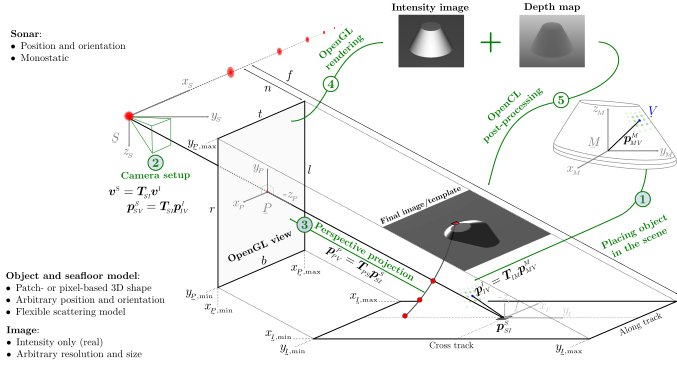
\includegraphics[width=\linewidth]{gfx/scene_coordinate_system.svg}%
\caption{Simulator principle. A model of the seafloor and object is first loaded into OpenGL, and an orthogonal camera view set up to match the desired image region on the seafloor. Then the scene is rendered and an intensity image and a depth map is created. The intensity image along with the depth information is finally combined to form a sonar like image. This is our template.}\label{simulator_coordinate_system}%
\end{figure*}

\begin{figure*}[t]\centering%
\includegraphics[drawing,width=\linewidth]{gfx/simulator.svg}%
\caption{Simulator concept.}\label{buildup}%
\end{figure*}

% \IEEEPARstart{W}{hen} 
% Autonomous underwater vehicles (AUVs). When an AUV with a sonar imaging system encounter an interesting object, it would be very beneficial if adapted its behavior to examine the object further. This is challenging as it would need to learn in what ways the interesting objects differ from the background, i.e. it relies on previous knowledge. It would also need to process this information is near real-time to act in an efficient manner.

% - Adapt simulation to its behaviour, see if they still match.

\IEEEPARstart{A}{utonomous} underwater vehicles (AUVs) are becoming increasingly important in human underwater endeavors. When equipped with a synthetic aperture sonar (SAS), they can e.g. be used to map the seafloor, survey underwater biology, help localize wrecks, inspect oil pipes, fields and electricity lines, or hunt for mines and biohazard waste. Such independent systems have much to gain from being able to adapt to the scenario at hand. For instance, with a well designed automatic target recognition (ATR) system on board they can adapt their mission plan to collect more information on particularly interesting objects, or fine-tune the sonar and navigation system to improve imaging performance.
 
% Automatic target recognition (ATR) is an important component in autonomous underwater vehicles (AUVs), as it allows the vehicle to adapt its mission plan to e.g. revisit detected objects for closer examination. One way to classify these objects is by using template matching. The principle involved  is to isolate an image segment containing the object of interest, compare it with a set of template images of the relevant object classes, and assign it to the class of the template with the the best fit.

In conventional ATR an object of interest is first isolated, its properties attempted estimated, and a classifier used to determine what object class these properties belong to. The challenge is finding unique and intrinsic object properties, such as its type, shape and size, and to do so independently of extrinsic properties such as its alignment, burial depth, degeneration level or view angle. While SAS provide images with state of the art resolution and dynamic range, they still only represent an ambiguous acoustical 2D projection of the 3D object, littered with a highly coherent noise floor. 

An alternative approach is to use template matching, where the isolated image segment is compared to a set of template images covering the relevant object classes, and assigned to the class of the template with the best fit. Since the templates are computed from 3D models, this reduces the issue of image ambiguity. However, a challenge is finding a set of templates that represent the actual configurations of object and seafloor, Another issue is that the size of precomputed library of templates grows exponentially with the number of parameters needed. This limits its use to only a few parameters being coarsely sampled, ultimately yielding inaccurate results~\cite{Midelfart2010}.


% We avoid the problems of conventional template matching by computing the templates on-the-fly as part of the classification process, thereby not needing a precomputed set of templates at all. 
%  that avoids this problem by running sufficiently fast to create templates adapted to the actual scene as part of the classification process.
% Classification process

We tackle the problems of conventional template matching by performing:
%
\begin{itemize}
\item \emph{Adaptive template matching}; where a template is selected based on object and seafloor parameters estimated from the SAS image~\cite{Midelfart2010}, and
\item \emph{Real-time template simulation}; where a template is created tailored to the estimated parameters, improving its accuracy and avoiding the need of a precomputed template library.
\end{itemize}
%

The methods presented herein will focus on the template simulator, but some details will also be given on adaptive template matching for completeness. More details on this technique can be found in~\cite{Midelfart2010}.


 This is achieved with the aid of the massive computing power in graphics processing units (GPUs) and optimized software libraries for scene rendering. The simulator loads a 3D model of the seafloor and object class into OpenGL and positions the camera at the sonar location. The scene is highlighted using a light tube that extends to infinity along the AUV's axis of probagation. We assume rough, isotropic surfaces reflecting sound energy equally in all directions. This can be modeled with a Lambertian scattering model~\cite{Blake1993,Bell1995}, where the intensity of the backscattered sound solely depends on the incidence angle of the transmitted signal onto the model surface. The OpenGL rendering produces an optical 2D intensity image and depth map that reveals the distance from each pixel to the propagation axis. For maximum flexibility this data is finally combined with OpenCL to produce the image templates.

as part of the classification process. This is achieved with the aid of the massive computing power in graphics processing units (GPUs) and optimized software libraries for scene rendering.

The simulator loads a 3D model of the seafloor and an object class model into OpenGL, where emitted sound waves are modeled with a cylindrical light source placed at the sonar transmit location. 

We assume rough, isotropic surfaces reflecting sound energy equally in all directions. This can be modeled with a Lambertian scattering model~\cite{Blake1993,Bell1995}, where the intensity of the backscattered sound solely depends on the incidence angle of the transmitted signal onto the model surface. When rendering OpenGL is set up to produce an optical 2D intensity image and depth map that reveals the distance from each pixel to the propagation axis. For maximum flexibility this data is finally combined with OpenCL to produce the image templates.

Various simulators for high frequency, side-looking sonar imagery have been published, e.g.~\cite{Bell1997,Sammelm2003}. However, most implementations have prioritized accurate acoustic modeling at the expense of execution speed. One exception is the SIGMAS+ simulator in~\cite{Coiras2009a, Coiras2009b}. Similarly to our approach it takes advantage of parallel processing on GPUs, and it uses OpenGL to render a 2D image from a 3D model, under the assumption of Lambertian scattering. However, SIGMAS+ is still aimed more towards realistically looking images, including effects like ambient noise, which is irrelevant for our purpose of template generation. Also, their simulator superimpose images obtained from multiple OpenGL rendering passes to create the sonar image, while we render once and post-process this result with OpenCL to tailor the sonar image with greater flexibility.


For lack of a better name, the simulator will be referred to as "FFISim" throughout this article.

Show:
\begin{itemize}
\item Adaptive template matching to avoid large static template libraries,
\item Improved classification performance by feeding simulator with parameters derived off SAS image,
\item Further improved classification by performing a fine-search within a narrow search space around the SAS derived parameters. GPU makes this more powerful.
\end{itemize}


\section{Methods}

Creating a 2D view of an arbitrary complex 3D scene is a non-trivial matter.  This is why we decided to use the core OpenGL pipeline to do this for us. OpenGL is a popular, well-matured and multi-platform application programming interface (API) for rendering 2D and 3D vector graphics. It relieves us from the intricacies of projecting vertices, faces and textures defined in a 3D space onto a suitable 2D image plane. This section explains how we set up OpenGL for this task, and then proceeds to describe how we post process the OpenGL images with OpenCL to form the final sonar image.

\begin{itemize}
\item Load arbitrary complex models
\item Simulate sonar with OpenGL
\item Speed considerations
\end{itemize}

Models are not ROCCAN (???)


\subsection{Loading the scene}

Our models are stored in regular 3D model files. The simulator begins by loading these into a tree of nodes, each representing a vertex in the model with corresponding facet and texture information. Then the vertices are placed into a virtual scene in OpenGL, and a camera set up to capture the part of the scene corresponding to the image. When OpenGL renders the image, it first computes which vertex contributes to which pixel in the image, then computes the intensity and color of the pixel based on the node's facet, texture and scattering model. The code that operates on vertices are called a vertex shader, and the code that operates on pixels are called a fragment shader.

Mapping of the vertices from object coordinates to image coordinates happen through a set of transformations:
%
\begin{align*}
\bmat{x\\y\\0\\1}_\text{image} = \boldsymbol{P} \cdot \boldsymbol{V} \cdot \boldsymbol{M} \cdot \bmat{x\\y\\z\\1}_\text{model},
\end{align*}
%
where $\bmat{\cdot}_\text{model}$ is the loaded model, $\bmat{\cdot}_\text{image}$ is the output image, and $\M$, $\V$ and $\P$ are model, view and transformation matrices, respectively. These will be described next.

The model matrix $\M$ is the first transform applied to the object, and is defined as:
%
\begin{align}
\M = \bmat{x_t \\ y_t \\ z_t \\ w}_\text{\parbox{1cm}{\setlength\baselineskip{0.3cm}transformed\\model}} &= \boldsymbol{T} \cdot \boldsymbol{R} \cdot \boldsymbol{S} \cdot \bmat{x \\ y \\ z \\ w}_\text{model},
\end{align}
%
where $\boldsymbol{S}$, $\boldsymbol{R}$ and $\boldsymbol{T}$ are transformation matrices\todo{be explicit on dependencies?} that sets the object's scale, rotation and translation, respectively. Combined these transforms map the object from its local coordinate system to the world's coordinate system. They are provided for reference in Appendix \ref{transformation_matrices}.

Next the object is mapped into world coordinates with the view matrix $\V$. This involves aligning the camera to precisely fit the image region. In our case the camera represents the phase center of the sonar, and it is placed in the world origin. The transformation then take the form of
%
\begin{align}
\V &= \mat{T}(x_\text{c}, y_\text{c}, z_\text{c}) \cdot \R_\text{x}(\phi_x, 0, 0) \nonumber\\
&= 
\bmat{
1  &  0  &  0  &  x_\text{c} \\
0  &  1  &  0  &  y_\text{c} \\
0  &  0  &  1  &  z_\text{c} \\
0  &  0  &  0  &  1 \\
} \cdot
\bmat{
1  &  0           &  0           &  0 \\
0  &  \cos\phi_x  &  -\sin\phi_x &  0 \\
0  &  \sin\phi_x  &  \cos\phi_x  &  0 \\
0  &  0           &  0           &  1 \\
},
\end{align}
%
where $(x_\text{c}, y_\text{c}, z_\text{c})$ is the image center coordinates for along track, cross track, and depth, respectively, and $\phi_x$ is the elevation angle\todo{is this correct?} of the sonar. It is given as
%
\begin{align*}
\phi_x &= \arctan\left(\frac{y_\text{mean}}{-z_\text{mean}}\right).
\end{align*}\todo{use absolute sign?}

Finally the relevant part of the scene is projected onto the image plane with a projection matrix $\P$. There are two main types of projection, perspective and orthographic. Perspective projection scales all $x$ and $y$ coordinates inversely with the distance to the objects to create a sense of perspective in the image. Orthographic projection, on the other hand, maps all the scene's vertices to a squared cube where each dimension has the range [-1,1]. This will render all objects equally large whether they are in the distance or up close. The matrix that gives orthographic projection is defined as
%
\begin{align}
\P = \left(\begin{matrix}
\frac{2}{r-l}  &  0              &  0              &  -\frac{r+l}{r-l} \\
0              &  \frac{2}{t-b}  &  0              &  -\frac{t+b}{t-b} \\
0              &  0              &  \frac{-2}{f-n} &  -\frac{f+n}{f-n} \\
0              &  0              &  0              &  1
\end{matrix}\right)
\end{align}
%
where $l,r,b$ and $t$ are the left, right, bottom and top boundaries of the projection plane, respectively, and where $n$ and $f$ is the near and far limits of the cube that encompass the scene. These parameters need to be adapted to provide a 2D image that matches the image size, which we specify in along track and cross track coordinates ($x,y$). This is straightforward for left and right since matches the $x$-axis
% They define the window through which we observe our scene.
\begin{align}
l &= x_\text{min}  &  r &= x_\text{max}
\end{align}
%
For the near and far limits one simply needs to make sure the scene will fit in it, say
%
\begin{align}
n &= 0\;\text{m}   &  f &= 300\;\text{m}.
\end{align}
%
The bottom and top boundaries can be inferred from \Fig{camera_top_bottom}. First we define an origin vector that points to the center of the image
%
\begin{align}
\vec o &= \left[\frac{x_\text{min}+x_\text{max}}{2}, \frac{y_\text{min}+y_\text{max}}{2}, \frac{z_\text{min}+z_\text{max}}{2} \right]\T,
\end{align}
%
and the distance from the image origin to its $y$-boundaries is given as
%
\begin{align}
\Delta y &= \frac{|y_\text{max} - y_\text{min}|}{2}.
\end{align}
%
To find the nearest and farthest point in the image that will be part of the projected scene, $\alpha$ and $\beta$, we must consider the seafloor rotation angle around the $x$-axis, $\Phi_x$ 
%
\begin{align}
\vec\alpha &= \vec 0 - \left[0, \Delta y, \Delta y \cdot \tan\Phi_\text{x} \right] \nn
\vec\beta &= \vec 0 + \left[0, \Delta y, \Delta y \cdot \tan\Phi_\text{x} \right]
\end{align}

\begin{figure}[t]\centering%
\includegraphics[drawing,width=\linewidth]{gfx/opengl_part.svg}%
\caption{Setting camera top and bottom boundaries.}\label{camera_top_bottom}%
\end{figure}



\subsection{OpenGL rendering}

To produce the sonar templates we assume a rough, isotropic surface that reflects energy equally in all directions. This permits us to use a Lambertian scattering model where the backscatter intensity depends only on the incidence angle~\cite{Zhang1999}. It does not consider observation angle or sound frequency, but for the purpose of creating templates this is not needed.   

The rendered image will appear as if we placed a window at the sonar and looked through it in the direction of the image. This window is resized to make sure that the template image perfectly fills it.

\subsection{OpenCL post-processing}

The ``camera image'' rendered with OpenGL is not in along-track and cross-track coordinates as we want it to be. It does, however, show us what parts of the scene that are visible from the sonar. OpenGL can also produce a depth map that reveals the distance to each of image pixels. This information can be converted to a ranged sonar-like image by simply adding up all the intensity values that share the same depth for each range line. We perform this computation in OpenCL. It allows general purpose programming on GPUs and can interoperate with OpenGL quite nicely. This way we keep all the calculations on the GPU.

\todo{
- Kernel tuning.
- Sharing. PBO. Asynchronous.
}

\subsection{Template matching}

1. Segmentation
2. Parameter estimation
   Available: Range, altitude, resolution => Input to both standard and adaptive. In standard the best fit out of a predefined template database is selected, then resampled to correct resolution.
   Additional for adaptive, parameters that modify object model: Target aspect angle, seafloor slope, object length and height.

   Target aspect angle computed with Radon Transform, seafloor under object modeled as plane with a slope estimated from bathymetric data, length estimated from longest part of highlight region, and height estimated from the shape of the shadow. The burial depth is n


   
3. 

   Details: \ref{Midelfart2010}.

Let $S(x,y)$ be the isolated part of the

Matching the isolated image segment with the template take the form of

\begin{align}
c_{h,i} = \underset{x',y'}{\text{argmax}} \sum\limits_{\forall x}\sum\limits_{\forall y} \big| H(x,y) - T(x-x',y-y') \big|
\end{align}

\begin{align}
c_i = \frac{c_{h,i} + c_{s,i}}{2}
\end{align}

And the final template used is the one with the greatest correlation coefficient

\begin{align}
\underset{T_i(x,y)}{\text{argmax}} C_i\sum\limits_{\forall x}\sum\limits_{\forall y}  S(x,y) T(x-x',y-y')
\end{align}

Then assign object to class $i$.


To narrow down the search space of possible templates we derive some reliable statistics of the seafloor and object from the SAS image. While FFISim accepts an arbitrarily complex seabed, we find that modeling it as a plane wave with the right tilt works well. The object is more difficult. For instance, we estimate its length and height from the shape of its shadow, but this fails if the object is notably immersed into the seabed at one end. 

After the a template is created we decompose it into its highlight and shadow component, and compute a correlation score between these and the corresponding areas in the SAS image. Then the two scores are summed and normalized to form the final correlation score of the template.

We tag the template matchers as either semi- or fully adaptive. The former refers to using the best matching SIGMAS+ generated template out of a precomputed set of templates, while the latter refers to the proposed method of using FFISim to generate templates on the-the-fly. \todo{Should be more precise. How many templates? Parameter span? How finely were the parameters sampled?} 

% It is also possible to compute the sonar image using the OpenGL ``blend'' feature.

\subsection{Speed considerations}

Using OpenGL and OpenGL to generate sonar templates on the GPU allow hundreds of sonar templates to be formed per second. While this is sufficient for our needs. However, initializing the OpenGL and OpenCL context and loading 3D models from file into it is a slow process, and typically takes several seconds for every invocation. Therefore, to alleviate the simulation performance we either had to supply it with a list of parameters or ensure that it did not have to be shut down for every invocation. 

The rendering loop that uses OpenGL and OpenCL to form 

\todo{
Write to file
}

%    """
%    
%    stm: Standard template matching, made with SIGMAS.
%    atm: Adaptive template matching, made with FFISim.
%    atm_bury: Adaptive template matching where a search of bury depths is used.
%    atm_bury_restr: Restricted?
%    
%    Adaptiveness made by letting the template matcher use 5 different rotation
%    angles in the ground-range axis. 
%    
%    
%    Data from Jesusbukta
%    
%    Figures are from run 2012.06.16
%    det210 - Cylinder 1: est 2.92m (short side towards sonar)
%    det233 - Cylinder 2: est 3.05m (diagonal)
%    det379 - Torpedo: est 5.06m (looks good)
%    
%    ROC curves from 3 different runs, first two just 2 days apart in 2009, last one in 2012.
%    
%    run_20120616 - last one. Much better with adaptive templates.
%    
%    ROC curves made by average correlation score of shadow/highlight from template matching.
%    
%    
%    fig4b(2015.11.16)
%       Bug that skipped masking of port side (negative y) detections past 180m range fixed
%       
%    fig4 (2015.11.16)
%       Bug leading to incorrect estimation of cylinder orientation fixed.
%          This affects run090601_1. Should be better after this.
%          
%    fig3 (2015.11.09)
%       Detections outside 180m range have been masked (but bug for port side fixed in fig4b).
%       Fixed an incorrectly annotated detection.
%       
%    fig2 (2015.11.02)
%       Height of object estimated from shadow length
%       Let adaptive method try 5 different rotations in ground-range (-4, -2, 0, 2, 4)
%          Improved results, but incorrect classification of:
%          5 detections in first run, and
%          3 detections in second run
%          => For FPR=0.2 the results are slightly worse than with normal adaptive (particularly first run).
%          Images are problematic in these cases:
%             2 detections get wrong orientation because a line (anchor) cross the image
%             Other misclassifications in image regions with poor echo or shadow strength
%          => Not a big issue as not enough time to detect more than ~20% of the detections in a run
%             In a MCM operation these detections would never be used.
%             The runs have 3000 detections each, photographing 20% of these is too much.
%          Performance FPR>0.2 not interesting.
%          Performance FPR<0.2 much better with adaptive template matching.
%          
%    fig (2015.10.23)
%       atm - cylinder orientation and length estimated from SAS image and fed into simulator.
%       
%       ROC curves from last run. Computing the mean correlation score of the shadow and highlight/echo.
%       Early results. Can only check vs. cylinder-like objects.
%       Standard template library created based on estimation of physical size of known cylinder mines.
%       Not possible for adaptive method to perform better when hitting such a target.
%       
%  
%    """

\section{Results \& Discussion}

\begin{figure*}[!tbp]\centering%
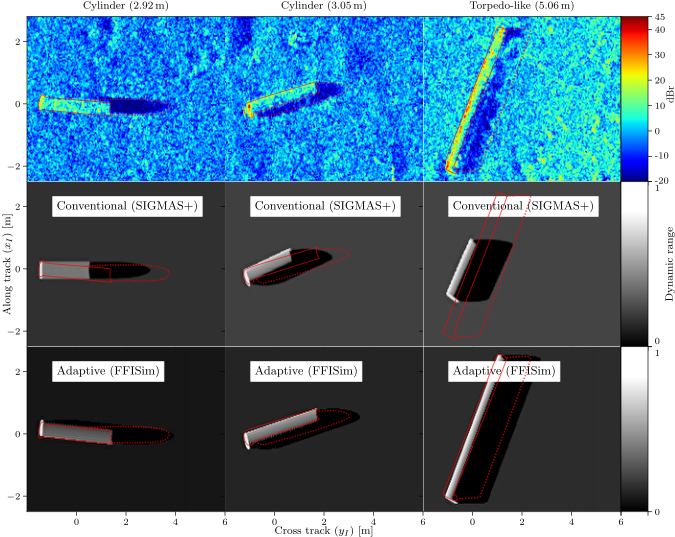
\includegraphics[width=\linewidth]{gfx/fig_images_sonar_simulator_tagged.svg}\label{fig_images_sonar_simulation}%
\caption{Selected objects. Top row show SAS images of 2 cylinders and a torpedo located in the Jesus Bay, Norway. Center row show the best match from a conventional template matcher, and bottom row show the adaptive template matcher. The contour of the SAS object is indicated with red lines. Note that the adaptive technique produce templates with a better fit to the highlight, but that this does not necessarily lead to a better match against the shadow.}
\end{figure*}

\begin{figure*}[!tbp]\centering%
\includegraphics[width=\linewidth]{gfx/fig_rocs.pdf}\label{fig_roc_curves}%
\caption{Receiver operating characteristics (ROC) curves.}
\end{figure*}

\begin{figure*}[!tbp]\centering%
\includegraphics[width=\linewidth]{gfx/fig_overlay.pdf}%
% \parbox{\linewidth}{\small\centering\vspace{.5\baselineskip}
% \newline\centering\newline %\\[.5\baselineskip]
\newcommand\cdesc[2]{{\raggedright\setlength\fboxsep{0pt}
\fbox{\colorbox[HTML]{#1}{\vrule height8.5pt depth3.5pt width0pt\hspace{.5cm}}}\ \ #2\\}}
\begin{minipage}{.4\linewidth}
\cdesc{800000}{Template highlight and image highlight}
\cdesc{FF1000}{Template highlight only}
\cdesc{FFEB00}{Image highlight only}
\cdesc{83FF7C}{Background pixels}
\end{minipage}%
\begin{minipage}{.4\linewidth}
\cdesc{000083}{Template shadow and image shadow}
\cdesc{0014FF}{Template shadow only}
\cdesc{00EFFF}{Image shadow only}
\cdesc{00A7FF}{Template shadow and image highlight}
\end{minipage}%}
\caption{Comparison of classification performance for the standard and adaptive template technique. The three objects were more or less arbitrary picked from the scene. For the roughly 3\,m long cylinders both methods perform similarly, the standard method seemingly with a slight edge. This is no surprise given that the 3\,m long cylinder model that make up the static template database fit the actual object well here. However, for the longer torpedo-like object the adaptive technique is clearly better. This is its merit; for objects and geometries that are not included in the static template database we can expect the adaptive techniques to perform better.}\label{fig_image_simulation}%
\end{figure*}

\newlength\imgspacing\setlength\imgspacing{.5cm}
\setcounter{topnumber}{2}

The performance of our simulator and template matching techniques where measured using experimental data from an interferometric HISAS1030 synthetic aperture sonar (SAS) attached to a HUGIN autonomous underwater vehicle (AUV), both developed by Kongsberg Maritime, Norway. The HISAS1030 is a fully digital phased array with 32 hydrophones, 100\,kHz center frequency and 30\,kHz bandwidth. It is 1.2\,m long, has a half-power beamwidth (HPBW) of 23$\circ$, and is capable of generating synthetic images with a theoretical resolution of 3-4\,cm in both dimensions. The version of HUGIN used also carries an camera that is used for optical inspection of interesting objects.

We present data from three different HUGIN runs from the Jesus Bay in Norway. The first two are taken a couple days apart in January 2009, containing roughly 2700 and 3200 detections, respectively. The last is from June 2012 and contains roughly 650 detections. The detections represent mostly cylinder shaped objects such as barrels, pipe mines and torpedoes. Therefore, all templates were based on a basic cylinder model.




The two template matchers can be visually inspected in \Fig{fig_images_sonar_simulator_tagged}. 

The classification performance is quantified with receiver operating characteristics (ROC) curves from all runs in \Fig{fig_roc_curves}. The 2009 runs proves a greater challenge than that from 2012, with 5 and 3 false positive detections at FPR=20\% in the January 6. and 8. run, respectively. This came as no surprise due to the 2009 runs containing fish trawler tracks and having poorer highlight and shadow quality than the run from 2012. However, for FPR<20\% the adaptive techniques outperform the static template library. For e.g. a mine counter measures (MCM) operation, this is the only region of interest because only a few objects out of the 3000 detections will be visually inspected up close.

- Stm stimulated with length matching test cylinder. Perfect score against this.
- Atm - not given to improve score. Shadow and highlight both need to match, and overfitting could lead to reduced performance.

In \Fig{fig_images_sonar_simulator_tagged} we compare the SAS image to the templates generated by the conventional and adaptive template matcher. Three typical objects from the 2012 were chosen, all being cylindric. The length two first being estimated to roughly 3\,m and the last 5\,m, likely representing cylinder mines and a torpedo, respectively. 

Selected objects. Top row show SAS images of 2 cylinders and a torpedo located in the Jesus Bay, Norway. Center row show the best match from a conventional template matcher, and bottom row show the adaptive template matcher. The contour of the SAS object is indicated with red lines. Note that the adaptive technique produce templates with a better fit to the highlight, but that this does not necessarily lead to a better match against the shadow.

Rotation around ground range axis: -4,-2,0,2,4 degrees.

Like the majority of objects in the Jesus Bay they are all cylinders with a length of a few meters. The same objects are simulated in \Fig{fig_image_simulation}, one with SIGMAS and the two other with FFISim. Each of these simulations were based on 





Good statistics drawn from the image -> adaptive better. Poor statistics -> hit and miss.




1. Comparison with standard template library (ROC enough?)
   ROC: Adaptive better at FPR<0.2 in all cases.
2. Comparison with SIGMAS
   Fairly similar images, performance is similar. 
   Used to create the standard template library.
3. Comparison with search space
   ROC: Additional search always better FPR<0.2.
   Explain search criterion.



SAS images - look good. Random pick objects. Lengths derived from image.
Simulated images - look good. Adaptive simulation more accurate. Otherwise similar. Different background level. Adaptive technique excels for less normal objects/geometries.
Overlap - Provide quantification measure. 


1. Adaptive better? Compare with standard. Doing this in ROC
2. Improved classification? ROCs
3. Further improvement by doing fine-search? ROC


An issue the adaptive technique must deal with when estimating object length 

As the ROC curves indicate, the adaptive template matching techniques both  ROC curves demonstrate the 

The majority of the objects in the Jesus Bay are cylinder shaped. A SAS image of three such objects are displayed in \Fig{fig_image_sonar}






% \begin{figure*}[!tbp]\centering%
% \subfloat[SAS images of 2 cylinders and a torpedo.]{%
% \includegraphics[width=0.5\linewidth]{gfx/fig_images_sonar_simulation.pdf}%
% \label{fig_sonar_simulation}}%
% \subfloat[Cylinder simulation with parameters estimated from SAS image: Length 2.6\;m, burial depth 0.263\;m, aspect angle 105$^\circ$.]{
% \includegraphics[drawing,width=0.5\linewidth]{gfx/sim_cylinder_submerged_adaptive.svg}%
% \label{sim_cylinder}}%
% \caption{A SAS image of a cylinder and a template simulation adapted to it.}
% \end{figure*}
% 
% 
% \begin{figure*}[!tbp]\centering%
% \subfloat[SAS image of a cylinder with 2.6\;m length and 0.53\;m radius.]{%
% 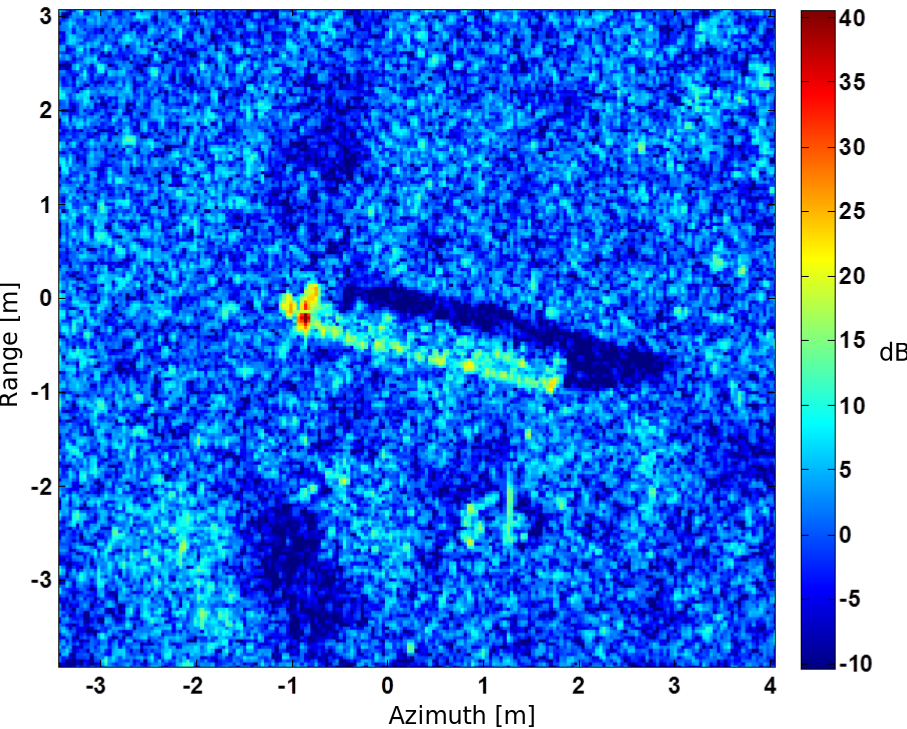
\includegraphics[drawing,width=0.5\linewidth]{gfx/data_cylinder_submerged.svg}%
% \label{data_cylinder}}%
% \subfloat[Cylinder simulation with parameters estimated from SAS image: Length 2.6\;m, burial depth 0.263\;m, aspect angle 105$^\circ$.]{
% \includegraphics[drawing,width=0.5\linewidth]{gfx/sim_cylinder_submerged_adaptive.svg}%
% \label{sim_cylinder}}%
% \caption{A SAS image of a cylinder and a template simulation adapted to it.}
% \end{figure*}


% \newcommand\cdesc[2]{#2}


% Whenever conventional computer graphics processing can be used to 
% GPUs are designed to provide the best possible graphics processing performance, and there large ecosystem of tools and libraries  available 
% Using a GPU to drive a simulator is advantageous since
% 
% 
% Creating a GPU-based simulator is attractive since computer is an attractive solution as there are a  graphics traits. For one over a CPU-based standard simulator is two-fold: 

Our GPU-based simulator is very fast. On a computer with a six-core Intel Core i7-3930K and a Radeon HD7970 it computes almost 1000 templates per second, each being 1 megapixel large. This makes it possible to tailor the templates very closely imaged objects. In contrast, in the standard approach a template library must be created beforehand from a limited set of parameter values. Hence, it may happen that no template in the library is a close fit of the object in the image even though the object actually is a target of interest.

This performance was demonstrated on an image from the HISAS 1030 synthetic aperture sonar mounted on the HUGIN AUV. Out of the objects in the scene we selected a 2.6\;m long cylinder that was partly buried in the sea sediments (Fig. \ref{data_cylinder}). The length, immersion depth and aspect angle of this cylinder were estimated from the SAS image using our  adaptive template matching approach~\cite{Midelfart2010}.  Then these parameters were used by the simulator to create an adaptive template (Fig. \ref{sim_cylinder}), which is an almost perfect match of the cylinder. We also created standard templates for a regular template matching approach. In this case, we assumed that the cylinder mine had a generic length of 2\;m (like a MP80 or a Murena mine) and was proud on the seafloor. Moreover, templates were created for every 10$^\text{th}$ degree of the aspect angle. We believe these assumptions to be typical for a template library for cylinder mines. 

The standard and adaptive templates were then matched to the HISAS image. This is illustrated in Fig. \ref{overlay_cylinder} for a standard template and in Fig. \ref{overlay_cylinder_adaptive} for an adaptive template. These images were created by segmenting the image and the templates into highlight, shadow, and background regions. The regions from a template were then laid on top of the regions of the image to illustrate how well these regions matched. Note how the adaptive template obtained a much closer fit to image than the standard template. This was also reflected in the correlation scores (which were created with the method described in \cite{Midelfart2010}) that were 0.613 for the standard template and 0.813 for the adaptive template. Hence, the standard approach was less likely to classify the cylinder in the image correctly as the standard templates were not created specifically for the target.

\begin{itemize}
\item GPUs low power. Good for integration in AUVs.
\item Good accuracy even with a real-time constraint in e.g. a AUV.
\item Improved inertial navigation?
\item Aid in understanding the key parts of the SAS image and in discovering potential flaws in the SAS image. Anomalies can be flagged to make SAS more robust?
\end{itemize}


\section{Conclusion}\label{conclusion}

One way to automatically classify objects in SAS images is to compare the imaged objects with a predefined set of templates. However, this is suboptimal as it is infeasible to create accurate templates for all the relevant configurations of seabeds and objects. To solve this we have implemented a SAS simulator that creates the templates in delayed real-time based on parameters estimated from the current scene. In our studies this improves the match between the SAS objects and their corresponding template significantly in most cases.

To obtain the delayed real-time performance we implemented the simulator on a GPU. These devices have a theoretical peak performance that is typically an order of magnitude higher than CPUs in a comparable price range. We found this potential to be effectively utilized with the well matured and highly optimized OpenGL graphics processing API. Our simulator use this framework for most of the scene processing.

A final post-processing step is performed in OpenCL, which allow general purpose GPU programming. It interoperates well with OpenGL and adds a lot of flexibility to the simulation process. This is valuable as the simulator is still being actively developed and will likely see new features that can not be easily implemented in OpenGL alone.

\begin{itemize}
\item Motion compensation
\item 
\end{itemize}

\ifPhdDoc
\clearpage
\appendix
\renewcommand\thesection{\Roman{section}}
\else
\appendices
\fi


\section{Transformation matrices}\label{transformation_matrices} 

Each data model that we load into OpenGL is defined in its own local coordinate system. To map them into OpenGL world coordinates a set of common transformation matrices are applied to each model's vertices:
%
\begin{align}
\bmat{x_t \\ y_t \\ z_t \\ w}_\text{\parbox{1cm}{\setlength\baselineskip{0.3cm}transformed\\model}} &= \boldsymbol{T} \cdot \boldsymbol{R} \cdot \boldsymbol{S} \cdot \bmat{x \\ y \\ z \\ w}_\text{model}.
\end{align}
%
Here a model vertex at position $(x,y,z)$ is first scaled with $\boldsymbol{S}$, then rotated with $\boldsymbol{R}$ and finally translated with $\boldsymbol{T}$, resulting in the transformed coordinates $(x_t,y_t,z_t)$. The parameter $w$ defines whether the vertex is a position ($w=1$) or a direction ($w=0$), which need to be handled differently. While these matrices are well-known in the field of computer graphics, there exist several different conventions but we supply them here for completeness.

The scaling and translation matrices are simple:
%
\begin{align}
\boldsymbol{S}(s_x,s_y,s_z) &= \bmat{
   s_x  &  0    &  0    &  0 \\
   0    &  s_y  &  0    &  0 \\
   0    &  0    &  s_z  &  0 \\
   0    &  0    &  0    &  1 \\
  },
  \end{align}
%
and

TZF64LJO2AUK2XEM
%
\begin{align}
\boldsymbol{T}(dx,dy,dz) &= \bmat{
	1  &  0  &  0  &  dx \\
	0  &  1  &  0  &  dy \\
	0  &  0  &  1  &  dz \\
	0  &  0  &  0  &  1 \\
},
\end{align}
%
where ($s_x$, $s_y$, $s_z$) and ($dx$, $dy$, $dz$) is scaling and translation factors.

Rotations will be specified using intrinsic Euler angles, i.e. as yaw ($\phi$), pitch ($\theta$) and roll ($\psi$), representing clockwise rotations around the $z$-, $y$- and $x$-axis, respectively. The Brian-Tait $Z$-$Y'$-$X''$ convention is used for rotation order, in which roll is applied first, then pitch and finally yaw:
%
\begin{align}
\R(\phi_x) = \R_z(\phi)\R_y(\theta)\R_x(\psi),
\end{align}
%
where
%
\begin{align}
\R_x(\psi) &= \bmat{
1  &  0           &  0           &  0 \\
0  &  \cos\psi  &  -\sin\psi &  0 \\
0  &  \sin\psi  &  \cos\psi  &  0 \\
0  &  0           &  0           &  1 \\
},
\end{align}
%
\begin{align}
\R_y(\theta) & = \bmat{
\cos\theta	& 0          & \sin\theta & 0 \\
0					& 1                   & 0          & 0          &  \\
-\sin\theta  & 0                   & \cos\theta & 0          &  \\
0            & 0                   & 0          & 1          &  \\
},           &
\end{align}
%
and
%
\begin{align}
\R_z(\phi) &= \bmat{
\cos\phi  &  -\sin\phi &  0  &  0 \\
\sin\phi  &  \cos\phi  &  0  &  0 \\
0				&  0           &  1  &  0 \\
0           &  0           &  0  &  1 \\
}.
\end{align}
%
Note that at $\theta=\frac{\pi}{2}$ we have $\phi=-\psi$, and at $\theta=-\frac{\pi}{2}$ we have $\phi=\psi$. Hence, one degree of freedom is lost at these points, an effect known as Gimbal lock. This can be solved by avoiding Eulean angles, e.g. by direct specification of orientation in terms of a rotation axis and angle. This can be achieved using the Euler-Rodrigues formula or with quaternions. The latter is the most common, due to added benefits such as reduced computational complexity, improved numerical stability and simple ways to perform spherical interpolations. However, in for our application this is not needed.
%
Translation is performed last. 
%




% \section{MVDR Complexity Formulas}\label{mvdr_formulas}
% 
% \section{GPU Throughput}\label{throughput}
% 
% bs bs

% use section* for acknowledgement
\ifCLASSOPTIONcompsoc% % This command fixes abstract positioning for compsoc articles:
% \IEEEdisplaynotcompsoctitleabstractindextext
% 
% % (Optional) Add some extra info on cover page of peer review papers:
% % \ifCLASSOPTIONpeerreview
% % \begin{center} \bfseries EDICS Category: 3-BBND \end{center}
% % \fi
% 
% % Insert page break and insert second title (peer review mode)
% \IEEEpeerreviewmaketitle
% 
% 
% 
  \section*{Acknowledgments}
\else
  \section*{Acknowledgment}
\fi


The authors would like to express their gratitude to the Norwegian Defence Research Establishment (FFI) for funding the development of the simulator.


% Can use something like this to put references on a page
% by themselves when using endfloat and the captionsoff option.
\ifCLASSOPTIONcaptionsoff
  \newpage
\fi

\ifPhdDoc
   \printbibliography[title=References,heading=subbibliography]
%    \bibliographysty
%    \bibliography{library.bib}
%    \print
\else
   \ifBuildBibliography
      \bibliographystyle{IEEEtran}
      \bibliography{references}

   \else
      % Paste here
   \fi

  
   % Generated by IEEEtran.bst, version: 1.13 (2008/09/30)
   % \begin{thebibliography}{10}
   % stuff here
   % \end{thebibliography}
   
   
   
\begin{IEEEbiography}[{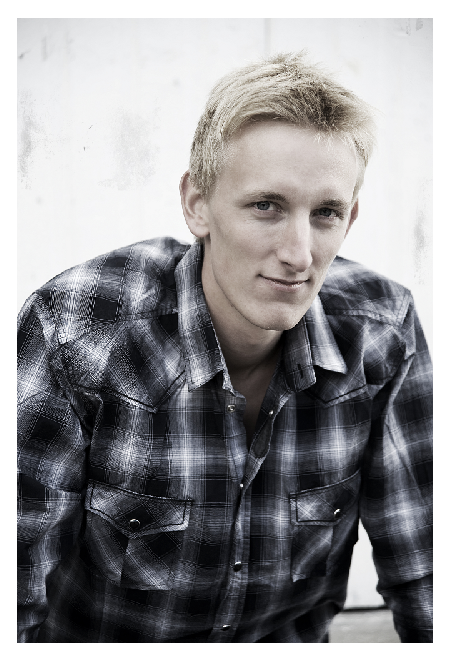
\includegraphics[width=1in,height=1.25in,clip,keepaspectratio]{bio/jo_inge.eps}}]{Jo Inge Buskenes}
received the B.Sc. degree in electrical engineering from Gj\o{}vik College University, Norway, in 2007, and the M.Sc. degree in instrumentation for particle physics from the University of Oslo, Norway, in 2010. He is currently pursuing the Ph.D. degree in acoustic image reconstruction and high performance computing at the University of Oslo.

His industry experience includes development of digital electronics at the European Organization for Nuclear Research (CERN), Geneva, Switzerland (2007-2008). He has lectured in digital signal processing at the Gj\o{}vik College University (2009), and at the University of Oslo (2010-2013). Current affiliation is with The Norwegian Defence Research Establishment, Kjeller, Norway, for which he is developing radar systems (2015-), and formerly sonar systems (2009, 2013).

His research interests include radar and sonar technology, adaptive image reconstruction, high performance computing, intelligent detector design and open source software.
\end{IEEEbiography}
   % 
\begin{IEEEbiography}[{
\includegraphics[width=1in,height=1.25in,clip,keepaspectratio]{bio/jon_petter.eps}}]{Jon Petter \AA{}sen}
(S'12) was born in Porsgrunn, Norway in 1986. He received the B.Sc. and M.Sc. degree in computer science from the University of Oslo, Norway, in 2010. He is currently pursuing his Ph.D. degree in medical ultrasound technology at the Norwegian University of Science and Technology (NTNU) Medical Imaging Lab (MI-Lab), Trondheim, Norway. His research interests include adaptive ultrasound processing techniques and acceleration of ultrasound algorithms using Graphics Processing Units (GPUs). 
\end{IEEEbiography}
   % 
\begin{IEEEbiography}[{
\includegraphics[width=1in,height=1.25in,clip,keepaspectratio]{bio/carl-inge.eps}}]{Carl-Inge Colombo Nilsen}
(S'06-M'10) received the M.Sc. and Ph.d. degrees in computer science from the University of Oslo, Norway, in 2005 and 2010. He is currently working at the University of Oslo as a postdoctoral research fellow. His research interests include signal and array processing for ultrasound imaging and other acoustical applications.
\end{IEEEbiography}
   % 
\begin{IEEEbiography}[{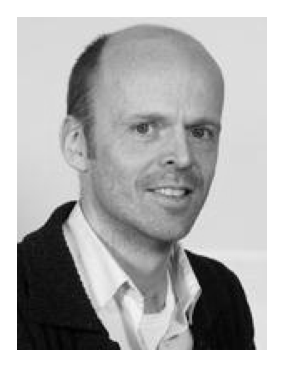
\includegraphics[width=1in,height=1.25in,clip,keepaspectratio]{bio/andreas.eps}}]{Andreas Austeng}
was born in Oslo, Norway, in 1970. He received the M.Sc. degree in physics in 1996 and the Ph.D. degree in computer science in 2001, both from the University of Oslo. Since 2001, he has been working at the Department of Informatics, University of Oslo, first as a postdoctoral research fellow and currently as an associate professor. His research interests include signal and array processing for acoustical imaging.
\end{IEEEbiography}
   
   
   % 
   % IMAGE METRICS
   %
   % - Point spread function (res via main lobe width, SAS gain via PDF height)
   % - Constrast measures
   %
   % ACR = cL/2
   % C = (s+n)/n ratio
   % - 
   % WHO's needing processing power
   % - Centre for Maritime Research and Experimentation
   
   
   \vfill 
   
   
\newpage 

\section{Rotation matrices}

If one accept the foundation of complex mathematics, the formulation of rotation matrices becomes apparent:
%
\begin{align}
\vec p_r(\theta_x)
&= \big(y +jz\big) \big( \cos\theta + j\sin\theta \big) \nn
&= \big(y\cos\theta - z\sin\theta ) +j\big( y\cos\theta + z\sin\theta \big) \nn
&= \bmat{ \cos\theta & -\sin\theta \\ \sin\theta & \cos\theta }\bmat{y \\ z}
\end{align}
%
\begin{align}
\vec p_r(\theta_y)
&= \big(x +jz\big) \big( \cos\theta - j\sin\theta \big) \nn
&= \big(x\cos\theta + z\sin\theta ) +j\big( x\cos\theta - z\sin\theta \big) \nn
&= \bmat{ \cos\theta & \sin\theta \\ -\sin\theta & \cos\theta }\bmat{x \\ z}
\end{align}
%
\begin{align}
\vec p_r(\theta_z)
&= \big(x +jy\big) \big( \cos\theta + j\sin\theta \big) \nn
&= \big(x\cos\theta - y\sin\theta ) +j\big( x\cos\theta + y\sin\theta \big) \nn
&= \bmat{ \cos\theta & -\sin\theta \\ \sin\theta & \cos\theta }\bmat{x \\ y}
\end{align}

\fi


\end{document}


